\documentclass[10pt]{beamer}
%\usetheme[
%%% option passed to the outer theme
%    progressstyle=fixedCircCnt,   % fixedCircCnt, movingCircCnt (moving is deault)
%]{}
  
% If you want to change the colors of the various elements in the theme, edit and uncomment the following lines

% Change the bar colors:
%\setbeamercolor{Feather}{fg=red!20,bg=red}

% Change the color of the structural elements:
%\setbeamercolor{structure}{fg=red}

% Change the frame title text color:
%\setbeamercolor{frametitle}{fg=blue}

% Change the normal text color background:
%\setbeamercolor{normal text}{fg=black,bg=gray!10}

%-------------------------------------------------------
% INCLUDE PACKAGES
%-------------------------------------------------------

\usepackage[utf8]{inputenc}
\usepackage[italian]{babel}
\usepackage{helvet}
\usepackage{listings}
\usepackage{xcolor}
\usepackage{graphicx}
\usepackage{multirow}
\usepackage{adjustbox}
\usepackage{booktabs}
\usepackage{subfig}
\usepackage{geometry}
\usepackage{tikz}
\usepackage{graphicx}

\usetikzlibrary{positioning,angles,quotes,calc,shapes.geometric}
\usetikzlibrary{chains,shapes.multipart}
\usetikzlibrary{shapes,calc,fit}
\usetikzlibrary{automata,positioning}


%-------------------------------------------------------
% DEFFINING AND REDEFINING COMMANDS
%-------------------------------------------------------

\usetheme{Frankfurt}

%-------------------------------------------------------
% INFORMATION IN THE TITLE PAGE
%-------------------------------------------------------

\title[Performance Modeling of Computer Systems and Networks] % [] is optional - is placed on the bottom of the sidebar on every slide
{ % is placed on the title page
      \textbf{Performance Modeling of Computer Systems and Networks}
}

\subtitle[ - Project 2018-2019]
{
      \textbf{Project 2018-2019}
}

\author[Andrea Graziani - 0273395]
{      Andrea Graziani - 0273395 \\
      {}
}

\institute[]
{
      Universit`a degli Studi di Roma “Tor Vergata” \\
      FACOLTA' DI INGEGNERIA \\
      Corso di Laurea Magistrale in Ingegneria Informatica
  
  %there must be an empty line above this line - otherwise some unwanted space is added between the university and the country (I do not know why;( )
}

\date{\today}

% ----------------------------------------------------------------------------------------- %
% Usato per personalizzare l'ambiente 'listings'...
% ----------------------------------------------------------------------------------------- %
\lstset{
language=C,
basicstyle=\tiny\ttfamily,			
keywordstyle=\color{blue},
commentstyle=\color{gray},			
stringstyle=\color{black},			
numbers=left,						
numberstyle=\tiny,					
stepnumber=1,						
breaklines=true						
}

%-------------------------------------------------------
% THE BODY OF THE PRESENTATION
%-------------------------------------------------------

\begin{document}

%-------------------------------------------------------
% THE TITLEPAGE
%-------------------------------------------------------

{% % this is the name of the PDF file for the background
\begin{frame}[plain,noframenumbering] % the plain option removes the header from the title page, noframenumbering removes the numbering of this frame only
  \titlepage % call the title page information from above
\end{frame}}







\section{System description}

\begin{frame}[fragile]{System description}{}

\begin{figure}[h!]
\resizebox{\columnwidth}{7.5cm}{%
\begin{tikzpicture}


% Cloud

\node[circle, draw, minimum width = 0.8cm]        					   (CloudNode0) at (0,2) {};
\node[circle, draw, minimum width = 0.8cm, below of=CloudNode0]        (CloudNode1) {};
\node[circle, draw, minimum width = 0.8cm, below of=CloudNode1]        (CloudNode2) {};
\node[circle, draw, minimum width = 0.8cm, below of=CloudNode2]        (CloudNode3) {};
\node[circle, draw=white, minimum width = 0.8cm, below of=CloudNode3]  (CloudNode4) {\rotatebox{90}{\textbf{....}}};

\node[above of=CloudNode4, yshift=-2.5cm, xshift=0.2cm] (labellllllll) {Cloud};

\node[right of=CloudNode0, xshift=-2.5cm] (ExtCloudNode0) {};
\node[right of=CloudNode1, xshift=-2.5cm] (ExtCloudNode1) {};
\node[right of=CloudNode2, xshift=-2.5cm] (ExtCloudNode2) {};
\node[right of=CloudNode3, xshift=-2.5cm] (ExtCloudNode3) {};


\coordinate (cloudStartNode) at (1.5,0);

% Controller

\node[circle, draw, minimum width = 2.2cm]  (ControllerExternal) at (4,0) {};
\node[circle, draw, minimum width = 2cm]    (Controller2)        at (4,0) {Controller};

\coordinate (cloudletStartNode) at (6.5,0);

\coordinate (Start) at (4,3.5);

% Cloudlet

\node[circle, draw, minimum width = 0.8cm, left of=ControllerExternal, xshift=5cm, yshift=2cm]       (CloudletNode0) {$1$};
\node[circle, draw, minimum width = 0.8cm, below of=CloudletNode0]           (CloudletNode1) {$2$};
\node[circle, draw, minimum width = 0.8cm, below of=CloudletNode1]           (CloudletNode2) {$3$};
\node[circle, draw=white, minimum width = 0.8cm, below of=CloudletNode2]     (CloudletNode3) {\rotatebox{90}{\textbf{....}}};
\node[circle, draw, minimum width = 0.8cm, below of=CloudletNode3] (CloudletNode4) {$N$};

\node[rectangle, draw, dashed, minimum width =6.5cm, minimum height=5.2cm] (Cloudlet) at (5.5,0) {};
\node[circle,below of=Cloudlet, yshift=-2cm, xshift=-1.5cm] (label1) {"One-hop" distance};

\node[left of=CloudletNode0, xshift=2.5cm] (ExtCloudletNode0) {};
\node[left of=CloudletNode1, xshift=2.5cm] (ExtCloudletNode1) {};
\node[left of=CloudletNode2, xshift=2.5cm] (ExtCloudletNode2) {};
\node[left of=CloudletNode4, xshift=2.5cm] (ExtCloudletNode3) {};

\node[rectangle, draw, dashed, minimum width =2cm, minimum height=5.5cm, right of=CloudletNode2, xshift=-1cm] (CloudletFrame) {};
\node[circle,above of=CloudletFrame, yshift=2.2cm] (label1) {Cloudlet Servers};

% Cloudlet Rows...

\draw[ultra thick,-] (ControllerExternal) -- (cloudletStartNode);
\draw[ultra thick,->] (cloudletStartNode) -- (CloudletNode0);
\draw[ultra thick,->] (cloudletStartNode) -- (CloudletNode1);
\draw[ultra thick,->] (cloudletStartNode) -- (CloudletNode2);
\draw[ultra thick,->] (cloudletStartNode) -- (CloudletNode4);

% Cloud Rows...

\draw[ultra thick,-] (ControllerExternal) -- (cloudStartNode);
\draw[ultra thick,->] (cloudStartNode) -- (CloudNode0);
\draw[ultra thick,->] (cloudStartNode) -- (CloudNode1);
\draw[ultra thick,->] (cloudStartNode) -- (CloudNode2);
\draw[ultra thick,->] (cloudStartNode) -- (CloudNode3);

% Out from cloudlet nodes

\draw[thick,->] (CloudletNode0) -- (ExtCloudletNode0);
\draw[thick,->] (CloudletNode1) -- (ExtCloudletNode1);
\draw[thick,->] (CloudletNode2) -- (ExtCloudletNode2);
\draw[thick,->] (CloudletNode4) -- (ExtCloudletNode3);

% Out from cloud nodes

\draw[thick,->] (CloudNode0) -- (ExtCloudNode0);
\draw[thick,->] (CloudNode1) -- (ExtCloudNode1);
\draw[thick,->] (CloudNode2) -- (ExtCloudNode2);
\draw[thick,->] (CloudNode3) -- (ExtCloudNode3);
 
% START

\draw[ultra thick,->] (Start) node[above] {Arrival Tasks} -- (ControllerExternal) ;

\node [cloud, right of=CloudNode3, xshift=-18, yshift=35, draw,cloud puffs=15,cloud puff arc=120, aspect=3, minimum width =2.5cm, minimum height=7cm, inner ysep=1em] (cloudcc) {};

\path (CloudletNode3) edge[->,dashed,ultra thick, bend left, out=0, in=170] node [left] [sloped, yshift=-5,xshift=60] {Interrupted jobs} (CloudNode4);

\end{tikzpicture}
}
\end{figure}

\end{frame}





\section{Specification model}
\subsection{Introduction}

% ************************************************************************** %
\begin{frame}{Specification model}{Introduction}


\begin{itemize}
\item What are the \textbf{state variables}?

\begin{table}[h!]
    \centering
    \small
    \begin{tabular}{p{1cm}p{0.5cm}p{8cm}}
       
      $n_x^{(c)}(\tau)$ & $ = $ & Number of class $c$ jobs currently running at $x$ system's node at time $\tau$ \\
      $d_x^{(c)}(\tau)$ & $ = $ & Number of class $c$ departed jobs from node $x$ at time $\tau$ \\
      $s_{x,i}^{(c)}$ & $ = $ & Service time of class $c$ job $i$ served on $x$ node   \\
      $i_{cloudlet}^{(2)}(\tau)$ & $ = $ & Number of class 2 interrupted jobs at time $\tau$ which were running on cloudlet (Access control algorithm 2 only!)\\
          
    \end{tabular}
\end{table}

Where:

\begin{table}[h!]
    \centering
    \small
    \begin{tabular}{l}
      $c \in \lbrace 1,2 \rbrace = C$ \\
      $x \in \lbrace cloudlet,cloud,global \rbrace = X$ \\
      $\tau \in (t_0, t)$ \\       
    \end{tabular}
\end{table}

\end{itemize}
\end{frame}

% ************************************************************************** %
\begin{frame}{Specification model}{Introduction}

\begin{itemize}
\item Are there any \textbf{constrains} regarding the values assumed by these variables?

\begin{equation}
\begin{array} {lr} 
\displaystyle \sum_{c \in C} n_{cloudlet}^{(c)}(\tau) \leq N & \forall \tau \in (t_0, t) \\\\
\end{array}
\end{equation}

\begin{itemize}
\item If you are using \textit{Access Control Algorithm 2}:

\begin{equation}
\begin{array} {rccr} 
n_{cloudlet}^{(2)}(\tau) > 0 & \Rightarrow & \displaystyle \sum_{c \in C} n_{cloudlet}^{(c)}(\tau) \leq S & \forall \tau \in (t_0, t) \\
S + 1 \leq n_{cloudlet}^{(1)}(\tau) \leq N & \Leftrightarrow & n_{cloudlet}^{(2)}(\tau) = 0 & \forall \tau \in (t_0, t)
\end{array}
\end{equation}
\end{itemize}

\end{itemize}

\end{frame}

% ************************************************************************** %
\subsection{System State}
\begin{frame}[fragile]{Specification Model}{System State}

\begin{itemize}
\item What's meant by \textbf{system state}?
\item So, how we can define system state formally?

\begin{equation}
\omega(\tau) = (\omega_{cloudlet}(\tau),\omega_{cloud}(\tau))
\end{equation}

Where:

\begin{equation}
\begin{array} {rcl} 
\omega_{cloudlet}(\tau) & = & (n_{cloudlet}^{(1)}(\tau),n_{cloudlet}^{(2)}(\tau)) \\
\omega_{cloud}(\tau) & = & (n_{cloud}^{(1)}(\tau),n_{cloud}^{(2)}(\tau)) \\
\end{array}
\end{equation}

Thus:

\begin{equation}
\begin{array} {rcl} 
\omega(\tau) = ((n_{cloudlet}^{(1)}(\tau),n_{cloudlet}^{(2)}(\tau)),(n_{cloud}^{(1)}(\tau),n_{cloud}^{(2)}(\tau))\\\\
\end{array}
\end{equation}

\item How do they evolve in time?
\end{itemize}

\end{frame}


% ************************************************************************** %
\subsection{Events}
\begin{frame}{Specification Model}{Events}

\begin{itemize}
\item What is an event?
\item What is the first event that can occur? And the last one?

\begin{equation}
\begin{array} {lr} 

n_x^{(c)}(t_0) = 0 & \forall c \in C, \forall x \in X \\\\
d_x^{(c)}(t_0) = 0 & \forall c \in C, \forall x \in X \\\\
n_x^{(c)}(t) = 0 & \forall c \in C, \forall x \in X \\\\
t_0 = 0, t = \tau^*
\end{array}
\end{equation}



\item So, what are the events capable to change system status?
\end{itemize}

\end{frame}

% ************************************************************************** %
\begin{frame}{Specification Model}{Events}

\begin{table}[h!]
    \begin{adjustbox}{center=\textwidth, height=105pt}
     \begin{tabular}{c|c|p{2.5cm}}

      \toprule
      \textbf{Event name that occurred at time $\tau$} & \textbf{Event's place} & \textbf{Event's effects} \\
      \midrule
      
      \multirow{3}{*}{Class 1 job arrival} & Cloudlet & $n_{\text{cloudlet}}^{(1)}(\tau)\texttt{++}$ \\ \cline{2-3} 
      & Cloud & $n_{\text{cloud}}^{(1)}(\tau)\texttt{++}$ \\ \cline{2-3} 
      & Controller & $n_{\text{global}}^{(1)}(\tau)\texttt{++}$ \\ 
       
      \hline
       
      \multirow{3}{*}{Class 2 job arrival} & Cloudlet & $n_{\text{cloudlet}}^{(2)}(\tau)\texttt{++}$ \\ \cline{2-3} 
      & Cloud & $n_{\text{cloud}}^{(2)}(\tau)\texttt{++}$ \\ \cline{2-3} 
      & Controller & $n_{\text{global}}^{(2)}(\tau)\texttt{++}$ \\ 
    
	  \hline
       
      \multirow{8}{*}{Class 1 job departure} & \multirow{4}{*}{Cloudlet} & $n_{\text{cloudlet}}^{(1)}(\tau)\texttt{--}$ \newline $n_{\text{global}}^{(1)}(\tau)\texttt{--}$ \newline $d_{\text{cloudlet}}^{(1)}(\tau)\texttt{++}$ \newline $d_{\text{global}}^{(1)}(\tau)\texttt{++}$ \\ \cline{2-3} 
      & \multirow{4}{*}{Cloud} & $n_{\text{cloud}}^{(1)}(\tau)\texttt{--}$ \newline $n_{\text{global}}^{(1)}(\tau)\texttt{--}$ \newline $d_{\text{cloud}}^{(1)}(\tau)\texttt{++}$ \newline $d_{\text{global}}^{(1)}(\tau)\texttt{++}$ \\ \cline{2-3} 
 
 		\hline
       
      \multirow{8}{*}{Class 2 job departure} & \multirow{4}{*}{Cloudlet} & $n_{\text{cloudlet}}^{(2)}(\tau)\texttt{--}$ \newline $n_{\text{global}}^{(2)}(\tau)\texttt{--}$ \newline $d_{\text{cloudlet}}^{(2)}(\tau)\texttt{++}$ \newline $d_{\text{global}}^{(2)}(\tau)\texttt{++}$ \\ \cline{2-3} 
      & \multirow{4}{*}{Cloud} & $n_{\text{cloud}}^{(2)}(\tau)\texttt{--}$ \newline $n_{\text{global}}^{(2)}(\tau)\texttt{--}$ \newline $d_{\text{cloud}}^{(2)}(\tau)\texttt{++}$ \newline $d_{\text{global}}^{(2)}(\tau)\texttt{++}$ \\
 
      \bottomrule


    \end{tabular}
    \end{adjustbox}
\end{table}

\end{frame}

% ************************************************************************** %
\begin{frame}{Specification Model}{Events}

\begin{itemize}
\item When you are using \textit{Access Control Algorithm 2}:

\begin{itemize}
\item If \textbf{class 1 job arrival event on controller} occurs:

\begin{equation}
n_{\text{global}}^{(1)}(\tau)\texttt{++}
\end{equation}

\item \textbf{If} following conditions are \textbf{all} true:

\begin{equation}
\begin{array} {rcl} 

n_{cloudlet}^{(1)}(\tau) & \neq & N \\\\

n_{cloudlet}^{(1)}(\tau) + n_{cloudlet}^{(2)}(\tau) & = & S \\\\

n_{cloudlet}^{(2)} & > & 0

\end{array}
\end{equation}

\textbf{Then}:

\begin{itemize}
\item $n_{cloudlet}^{(2)}(\tau)--$
\item Class 1 job arrival on cloudlet node event is scheduled.
\item Class 2 job arrival on cloud node event is scheduled.
\item A Class 2 job departure on cloudlet node event is removed from the \textit{event list}.
\item $i_{cloudlet}^{(2)}(\tau)++$
\end{itemize}

\end{itemize}


\end{itemize}
\end{frame}

% ************************************************************************** %

\subsection{computation}
\begin{frame}{Specification Model}{Statistics computation}

\begin{itemize}
\item How to compute requested statistics?


\begin{equation}
\begin{array} {rclr} 
E[N_x]^{(c)} & = & \displaystyle  \dfrac{1}{t-t_0}\int_{t_0}^t n_x^{(c)}(\tau)d\tau & \qquad \forall c \in C, \forall x \in X
\end{array}
\end{equation}

\begin{equation}
\begin{array} {rclr} 
E[N_x] & = & \displaystyle  \dfrac{1}{t-t_0} \cdot \int_{t_0}^t \left( n_x^{(1)}(\tau) + n_x^{(2)}(\tau) \right) d\tau \\\\
	   & = & \displaystyle  \dfrac{1}{t-t_0} \cdot \int_{t_0}^t n_x^{(1)}(\tau)d\tau + \dfrac{1}{t-t_0} \cdot \int_{t_0}^t n_x^{(2)}(\tau)d\tau \\\\
	   & = & E[N_x]^{(1)} + E[N_x]^{(2)} \\\\
	   & = & \displaystyle  \sum_{c \in C} E[N_x]^{(c)} & \forall x \in X
\end{array}
\end{equation}

\end{itemize}
\end{frame}

% ************************************************************************** %
\begin{frame}{Specification Model}{Statistics computation}

\begin{equation}
\begin{array} {rccccr} 
E[T_x]^{(c)} & = & E[S_x]^{(c)} & = & \displaystyle \dfrac{1}{d_x^{(c)}(t)} \cdot \sum_{i = 0}^{d_x^{(c)}(t)} s_{x,i}^{(c)} & \forall c \in C, \forall x \in X \\
\end{array}
\end{equation}

\begin{equation}
\begin{array} {rccccr} 
E[T_x] & = & E[S_x] & = & \displaystyle \dfrac{1}{d_x^{(1)}(t) + d_x^{(2)}(t)} \cdot \left( \sum_{i = 0}^{d_x^{(1)}(t)} s_{x,i}^{(1)} + \sum_{i = 0}^{d_x^{(2)}(t)} s_{x,i}^{(2)} \right) & \forall x \in X \\
\end{array}
\end{equation}


\end{frame}


\section{Computational Model}


\subsection{Next-event simulation logic}

% ************************************************************************** %
\begin{frame}{Computational Model}{Next-event simulation logic}

\begin{itemize}
\item Which are main features of a discrete-event simulation using a \textbf{next-event} approach?

\item How we have implemented \textit{simulation clock} and the \textit{event list}?

\item How we have implemented next-event simulation algorithm in our computational model?
\end{itemize}

\end{frame}

% ************************************************************************** %
\begin{frame}[fragile]{Computational Model}{Next-event simulation logic}

\begin{lstlisting}[frame=lines, caption={\texttt{ComputationalModel.perform} method}]
public void perform() {

   initializeSimulation();
   
   while (!this.simulationEventList.isEmpty()) {

      SimulationEvent actualEvent = this.simulationEventList.poll();

      if (actualEvent != null) {

          SimulationClock.getInstance().setCurrentEventTime(actualEvent.getStartTime());

          actualEvent.perform();
          actualEvent.scheduleFollowingEvent();

          SimulationEvent nextEvent = this.simulationEventList.peek();

          if (nextEvent != null)
              SimulationClock.getInstance().setNextEventTime(nextEvent.getStartTime());
      }
      updateStatistics();
   }
...
\end{lstlisting}

\begin{lstlisting}[frame=lines, caption={\texttt{ComputationalModel.initializeSimulation} method}]
private void initializeSimulation() {
     initializeSystemStateVariables();
     initializeSimulationClock();
     scheduleInitialEvent();
}
\end{lstlisting}
\end{frame}


% ************************************************************************** %
\begin{frame}[fragile]{Computational Model}{Next-event simulation logic}


\begin{lstlisting}[frame=lines, caption={\texttt{System} class methods}]
@Override
protected void initializeSystemStateVariables() {
    this.cloud.initializeSystemStateVariables();
    this.cloudlet.initializeSystemStateVariables();
    this.globalNetwork.initializeSystemStateVariables();
}

@Override
protected void initializeSimulationClock() {
    SimulationClock.getInstance().setCurrentEventTime(0.0);
    SimulationClock.getInstance().setNextEventTime(0.0);
}

@Override
protected void scheduleInitialEvent() {
    this.globalNetwork.scheduleInitialEvent();
}
\end{lstlisting}

\begin{lstlisting}[frame=lines, caption={\texttt{GlobalNetwork.scheduleInitialEvent} method}]
@Override
public void scheduleInitialEvent() {
    SystemEvent firstEventClass1 = SystemEventFactory.buildClass1JobArrival();
    SystemEvent firstEventClass2 = SystemEventFactory.buildClass2JobArrival();

    this.system.scheduleEventOnGlobalNetwork(firstEventClass1, this.getNextClass1JobInterArrivalTime());
    this.system.scheduleEventOnGlobalNetwork(firstEventClass2, this.getNextClass2JobInterArrivalTime());
}
\end{lstlisting}
\end{frame}



\subsection{Events}
\begin{frame}{Computational Model}{Events}

\begin{itemize}
\item How we have implemented events in our computational model?
\end{itemize}
\end{frame}


% ************************************************************************** %
\subsection{Next-event simulation logic}
\begin{frame}{Computational Model}{Events}
\begin{figure}
\centering
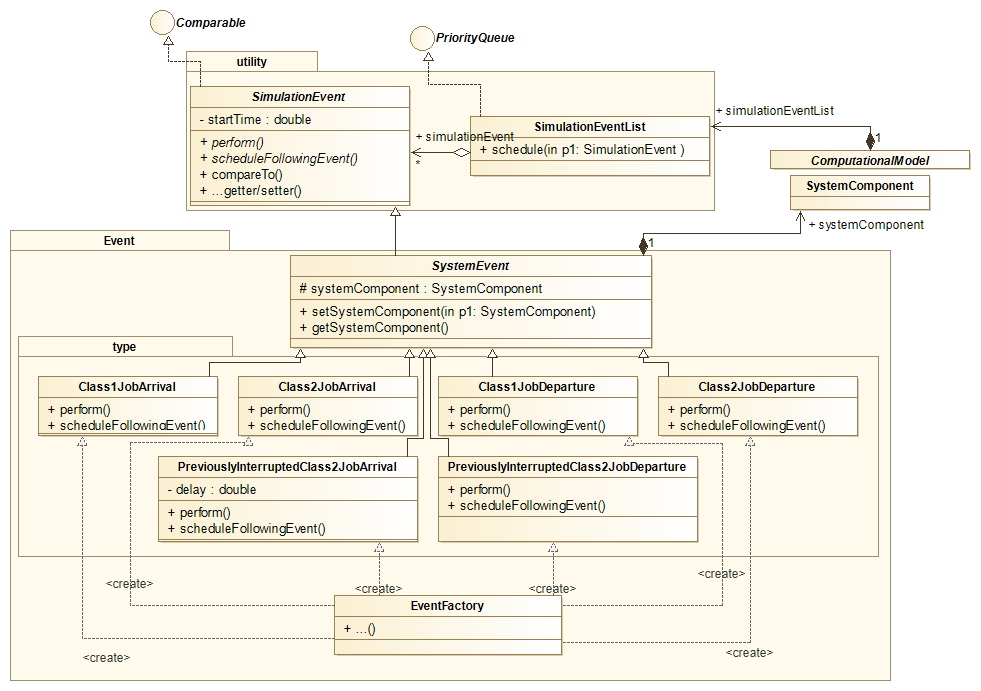
\includegraphics[width=\textwidth]{./images/ClassDiagramEvent.png}
\label{fig:Concorrente}
\end{figure}
\end{frame}


% ************************************************************************** %
\begin{frame}[fragile]{Computational Model}{Events}

\begin{lstlisting}[frame=lines, caption={\texttt{SystemEvent} class}]
public abstract class SystemEvent extends SimulationEvent {

    protected SystemComponent systemComponent;

    public void setSystemComponent(SystemComponent systemComponent) {
        this.systemComponent = systemComponent;
    }

    public SystemComponent getSystemComponent() {
        return systemComponent;
    }
    ...
}
\end{lstlisting}

\begin{lstlisting}[frame=lines, caption={\texttt{Class1JobArrival} class}]
public class Class1JobArrival extends SystemEvent {

    @Override
    public void perform() {
        this.systemComponent.updateStatusAfterClass1JobArrival();
    }

    @Override
    public void scheduleFollowingEvent() {
        this.systemComponent.scheduleFollowingEventAfterClass1JobArrival();
    }
}
\end{lstlisting}
\end{frame}

\begin{frame}[fragile]{Computational Model}{Events}

\begin{itemize}
\item \texttt{PreviouslyInterruptedClass2JobArrival}? What is it for?
\end{itemize}


\begin{lstlisting}[frame=lines, caption={\texttt{PreviouslyInterruptedClass2JobArrival} class}]
public class PreviouslyInterruptedClass2JobArrival extends SystemEvent {

    private double delay;

    public PreviouslyInterruptedClass2JobArrival(double delay) {
        this.delay = delay;
    }

    @Override
    public void perform() {
        this.systemComponent.updateStatusAfterPreviouslyInterruptedClass2JobArrival(this.delay);
    }

    @Override
    public void scheduleFollowingEvent() {
        this.systemComponent.scheduleFollowingEventAfterPreviouslyInterruptedClass2JobArrival();
    }
}
\end{lstlisting}
\end{frame}











% ************************************************************************** %
\subsection{System implementation}
\begin{frame}{Computational Model}{System implementation}

\begin{itemize}
\item How we have implemented our system? 
\item Which classes hold system state variables? Which compute output statistics?
\item How can we start our simulator?
\end{itemize}
\end{frame}

% ************************************************************************** %
\begin{frame}{Computational Model}{System implementation}
\begin{figure}
\centering
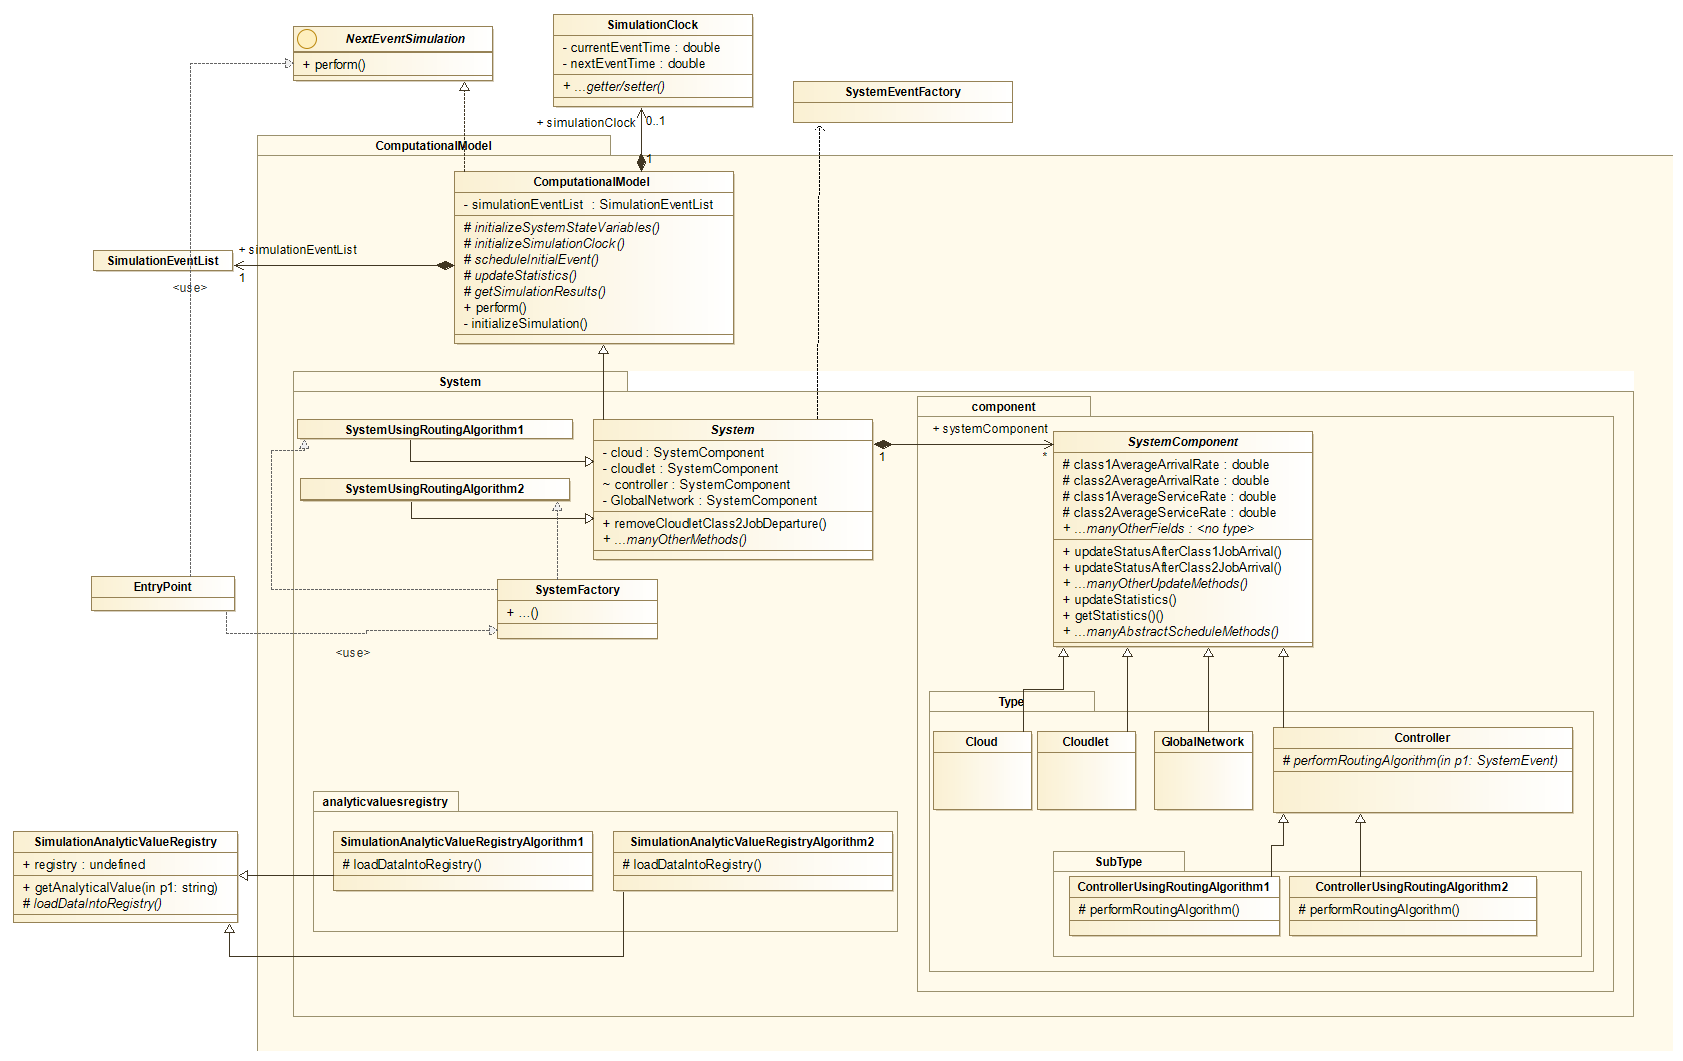
\includegraphics[width=\textwidth]{./images/ClassDiagram.png}
\label{fig:Concorrente}
\end{figure}
\end{frame}


\subsection{Class 2 job interruption}
\begin{frame}{Computational Model}{Class 2 job interruption}

\begin{itemize}
\item How we manage class 2 job interruption?
\end{itemize}
\end{frame}

% ************************************************************************** %

\begin{frame}[fragile]{Routing algorithm 2}{Class 2 job interruption}

\begin{lstlisting}
protected void performRoutingAlgorithm(SystemEvent event) {

    int n1 = this.system.getNumberOfClass1JobOnCloudlet();
    int n2 = this.system.getNumberOfClass2JobOnCloudlet();

        if (event instanceof Class1JobArrival) {

            if (n1 == this.system.getThreshold())
                this.system.scheduleEventOnCloud(event, 0);
            else if (n1 + n2 < this.system.getThreshold())
                this.system.scheduleEventOnCloudlet(event, 0);
            else if (n2 > 0) {

                double runningCloudletTimeOfInterruptedJob = this.system.removeCloudletClass2JobDeparture();

                this.system.scheduleEventOnCloudlet(event, 0);

                double setupTime = RandomNumberGenerator.getInstance().getExponential(5, 0.8);

                this.system.scheduleEventOnCloud(SystemEventFactory.buildPreviouslyInterruptedClass2JobArrival(setupTime + runningCloudletTimeOfInterruptedJob), setupTime);

                this.numberOfInterruptedClass2Jobs++;

            } else
                this.system.scheduleEventOnCloudlet(event, 0);


        } else {

            ...
        }
    }
\end{lstlisting}
\end{frame}


\section{Statistics Results}

% ----------------------------------------------------------------------------------------- %
\subsection{Finite-Horizon}
\begin{frame}{Statistics Results}{A Finite-Horizon simulation}

\begin{itemize}
\item What kind of simulation have we performed?
\item What is generated at the end of each simulation? How we can provide an estimation for required metrics?

Let $i$ i-th replication, where $i = 0,...,n$

\begin{equation}
\bar{x_i}(t) = \int_0^t x_i(t)dt \qquad \forall i=1,...,n
\end{equation}

\begin{equation}
E[\bar{x}(t)] = \dfrac{1}{n} \sum_{i=1}^n \bar{x_i}(t)
\end{equation}

Obliviously, interval estimate for $E[\bar{x}(t)]$ can be calculated from the ensemble mean and standard deviation.

\end{itemize}

\end{frame}

\begin{frame}[fragile]{Statistics Results}{Il processo client}


\begin{figure}
\centering
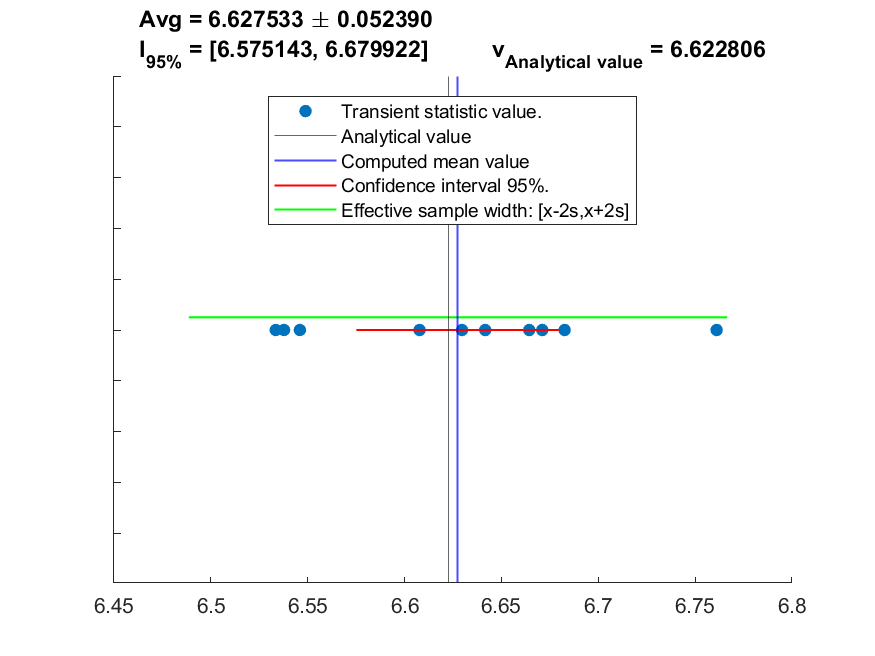
\includegraphics[width=\textwidth]{./images/EnsembleStatisticsCloud_Class1JobsNumber.png}
\end{figure}

\end{frame}




\subsection{Steady state}
\begin{frame}{Statistics Results}{A Finite-Horizon simulation}

\begin{itemize}

\item What are steady-state statistics? When they exist?
\item So, do the steady-state statistics exist in our system?
\item Is possible to obtain an interval estimation for steady state statistics using our simulator?
\end{itemize}

\end{frame}

% ----------------------------------------------------------------------------------------- %
\begin{frame}{Statistics Results}{Steady State statistics}

\begin{figure}
\centering
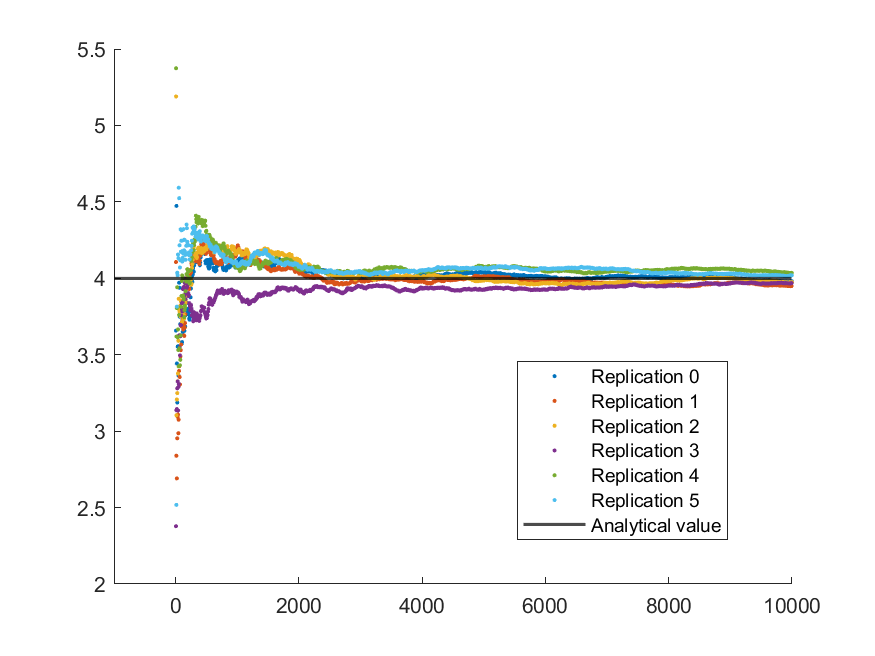
\includegraphics[width=\textwidth]{./images/ScatterPlotCloud_Class1JobsServiceTime.png}
\caption{Class 1 Jobs Service Time}
\label{fig:Concorrente}
\end{figure}
\end{frame}

\begin{frame}{Statistics Results}{Steady State statistics}

\begin{itemize}
\item Finite-horizon interval estimates are accurate steady-state estimates, becoming increasingly more accurate as the number of jobs increases.

\item The steady-state average wait indicator is interior to the finite-horizon interval estimate, suggesting that current system simulation parameters ($\tau^*$, $n$) allow us to achieve statistics that are close to their steady-state values.

\item But there is another way...

\end{itemize}
\end{frame}


\section{Routing Algorithms Comparison}
\begin{frame}[fragile]{Access control algorithms comparison}{}

\begin{itemize}
\item Which routing policy is better?
\end{itemize}

\begin{figure}
    \centering
    \subfloat[Cloudlet]{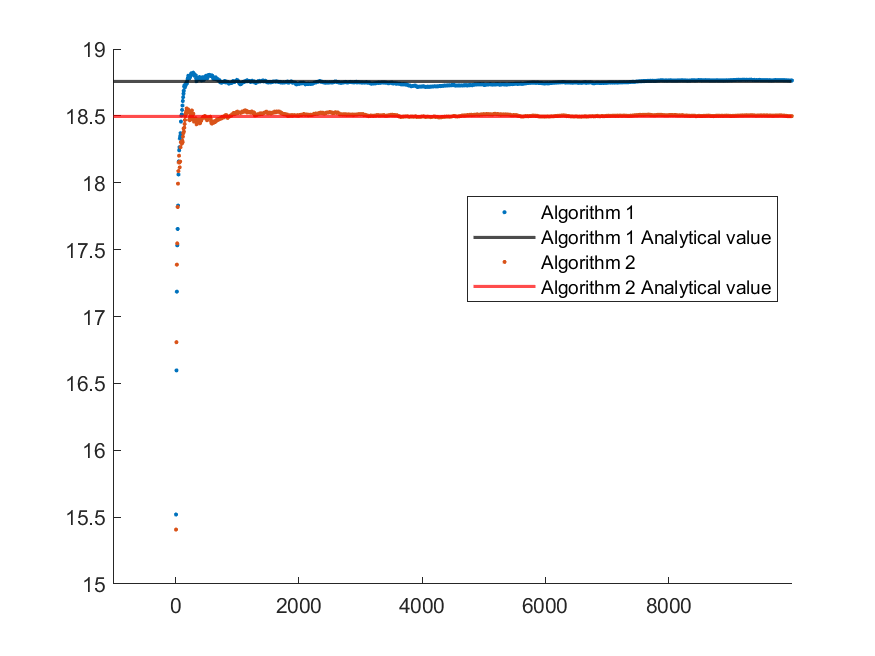
\includegraphics[width=3.6cm]{./Compare/ScatterPlotCloudlet_JobsNumber.png}}   
    \subfloat[Cloud]{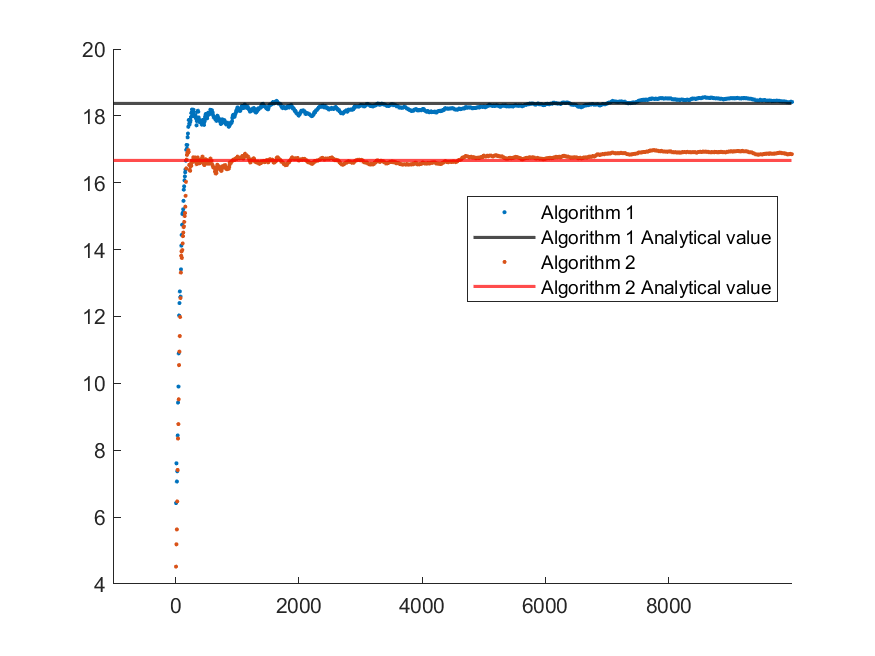
\includegraphics[width=3.6cm]{./Compare/ScatterPlotCloud_JobsNumber.png}}
    \subfloat[Global]{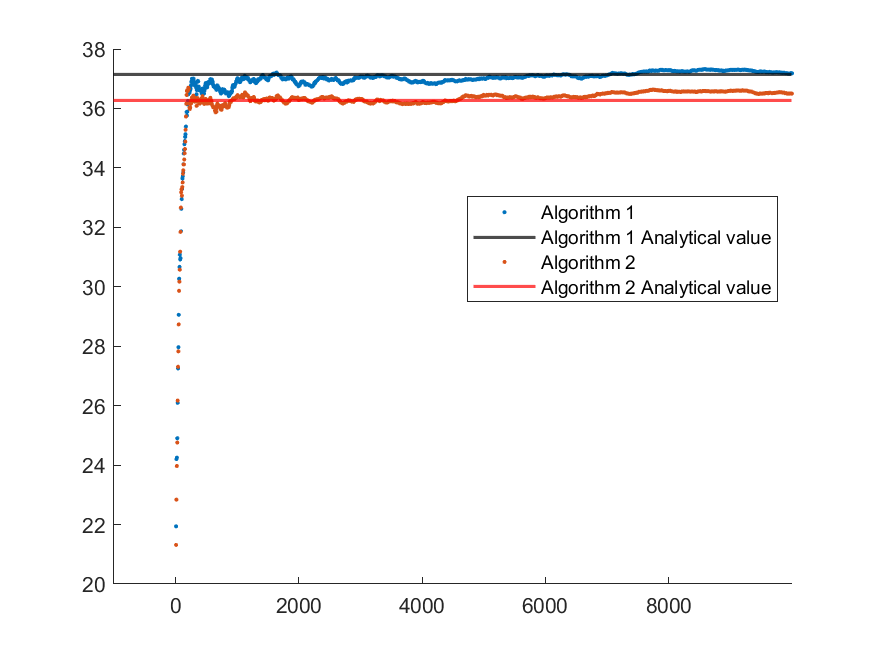
\includegraphics[width=3.6cm]{./Compare/ScatterPlotGlobalNetwork_JobsNumber.png}}
    \caption{Time-Average Job Population}%
\end{figure}



\end{frame}

\begin{frame}[fragile]{Access control algorithms comparison}{}

\begin{figure}[h!]
    \centering
    \subfloat[Class 1 Jobs]{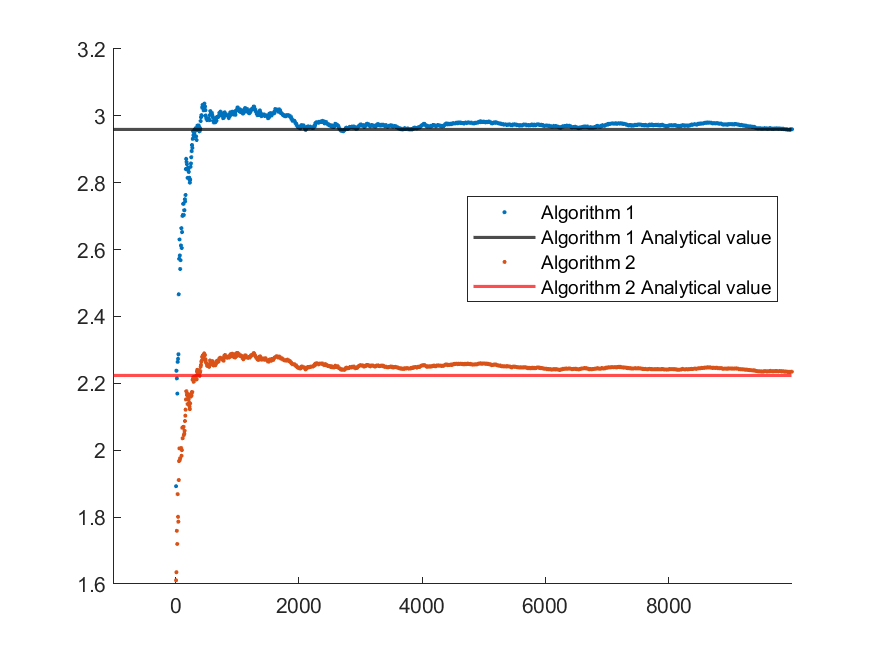
\includegraphics[width=3.6cm]{./Compare/ScatterPlotGlobalNetwork_Class1JobsServiceTime.png}}
    \subfloat[Class 2 Jobs]{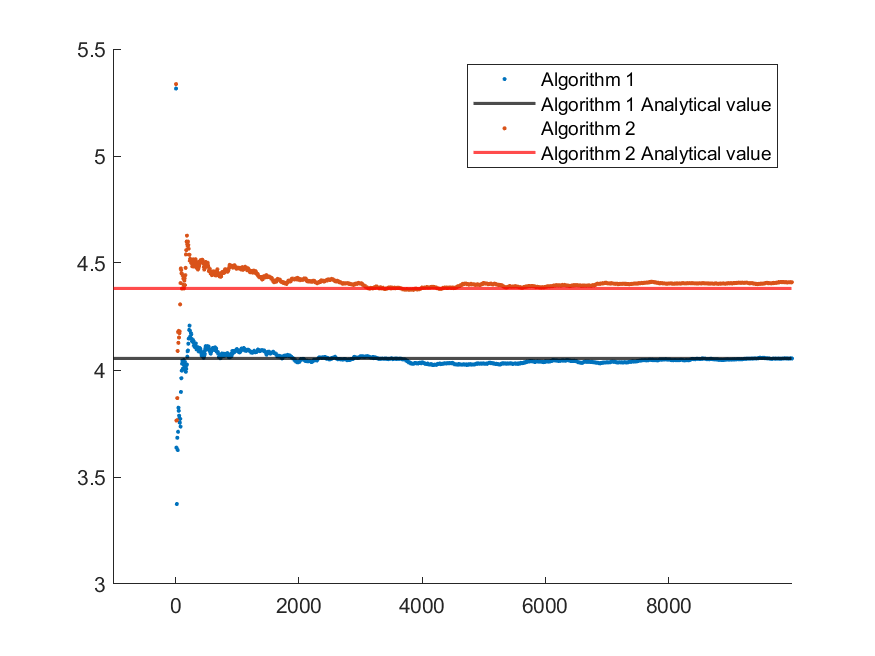
\includegraphics[width=3.6cm]{./Compare/ScatterPlotGlobalNetwork_Class2JobsServiceTime.png}}
    \subfloat[Both Classes]{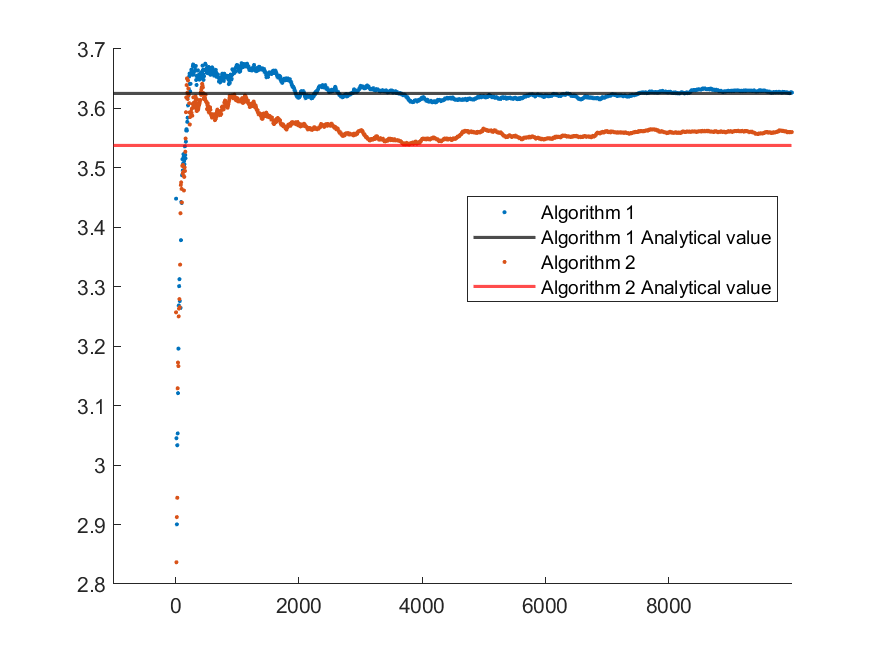
\includegraphics[width=3.6cm]{./Compare/ScatterPlotGlobalNetwork_JobsServiceTime.png}}
    \caption{Global Time-Average service/response time}%
\end{figure}

\end{frame}


\begin{frame}[fragile]{Access control algorithms comparison}{}
\begin{figure}[h!]
    \centering
    \subfloat[]{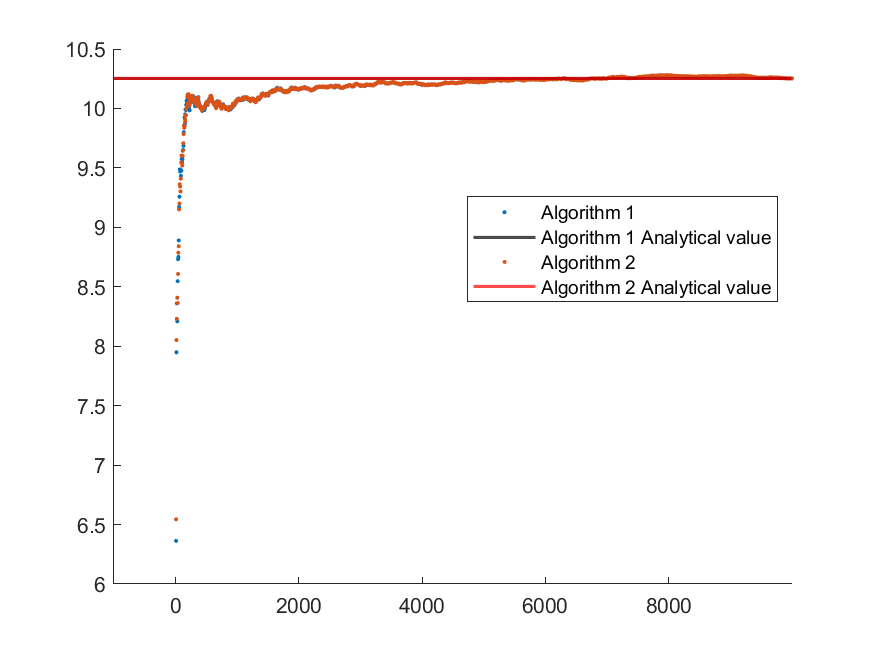
\includegraphics[width=7cm]{./Compare/ScatterPlotGlobalNetwork_Throughput.png}}
    \caption{Global Throughput}%
\end{figure}
\end{frame}

\begin{frame}[fragile]{Access control algorithms comparison}{}
\begin{figure}[h!]
    \centering
    \subfloat[Class 1 Jobs]{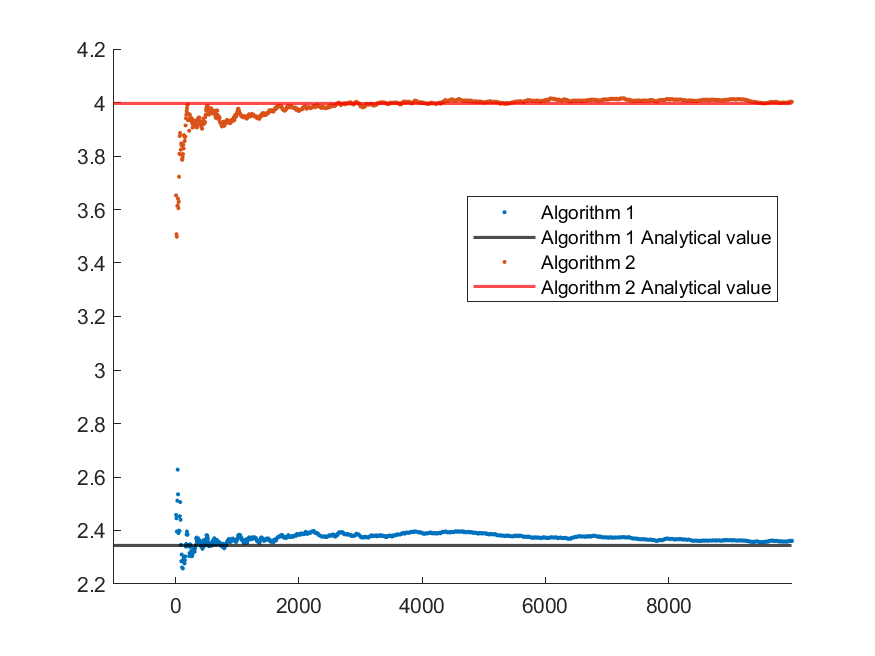
\includegraphics[width=3.6cm]{./Compare/ScatterPlotCloudlet_Class1Throughput.png}}
    \subfloat[Class 2 Jobs]{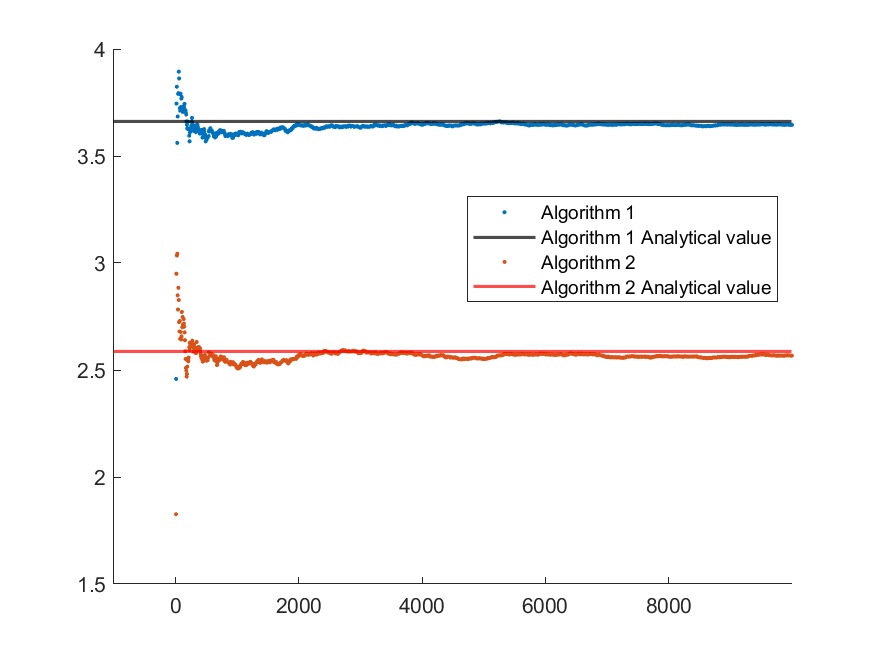
\includegraphics[width=3.6cm]{./Compare/ScatterPlotCloudlet_Class2Throughput.png}}
    \subfloat[Both Classes]{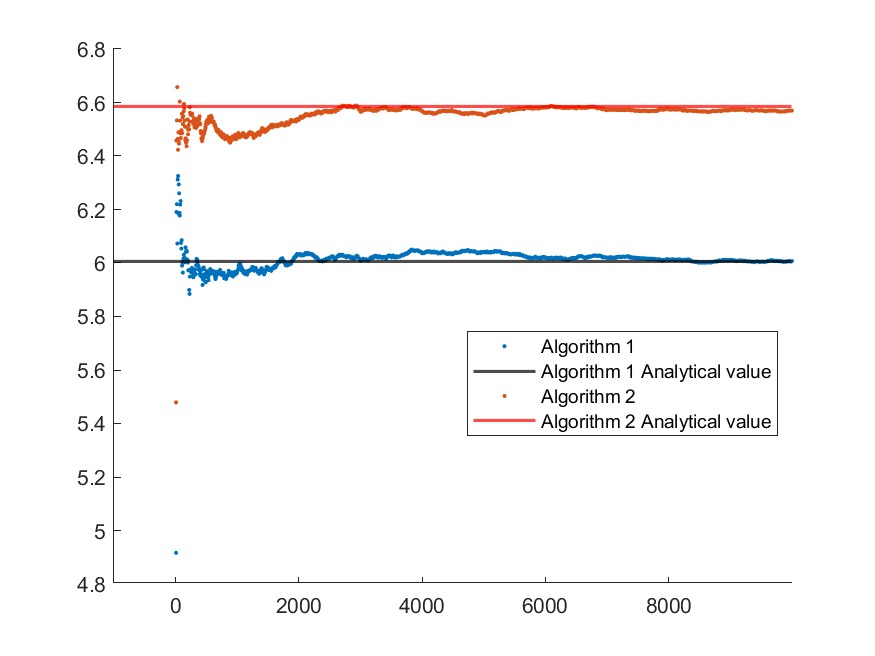
\includegraphics[width=3.6cm]{./Compare/ScatterPlotCloudlet_Throughput.png}}
    \caption{Cloudlet Throughput}%
\end{figure}
\end{frame}


\begin{frame}[plain,noframenumbering]
  Grazie per l'attenzione!
\end{frame}


\end{document}